\documentclass{beamer}
\usetheme{Singapore}
\usepackage{changepage}

%\usepackage{pstricks,pst-node,pst-tree}
\usepackage{amssymb,latexsym,dirtree}
\usepackage{tikz}
\usepackage{graphicx}
\usepackage{fancyvrb}
%\usepackage{hyperref}
\usepackage{fancybox}
\usepackage[listings]{tcolorbox}

\definecolor{codegreen}{rgb}{0,0.6,0}
\definecolor{codegray}{rgb}{0.5,0.5,0.5}
\definecolor{codepurple}{rgb}{0.58,0,0.82}
\definecolor{backcolour}{rgb}{0.95,0.95,0.92}

\lstdefinestyle{mystyle}{
    language=Python,
    backgroundcolor=\color{backcolour},   
    commentstyle=\color{codegreen},
    keywordstyle=\color{magenta},
    numberstyle=\tiny\color{codegray},
    stringstyle=\color{codepurple},
    basicstyle=\ttfamily\normalsize,
    breakatwhitespace=false,         
    breaklines=true,                 
    captionpos=b,                    
    keepspaces=true,                 
    numbers=left,                    
    numbersep=5pt,                  
    showspaces=false,                
    showstringspaces=false,
    showtabs=false,                  
    tabsize=2,
    escapechar=|,
    frame=single
}

\lstset{style=mystyle}


\newcommand{\lst}[1]{\lstinline{#1}}

\newcommand{\lsting}[1]{\begin{lstlisting}[basicstyle=#1]}
\newcommand{\lstend}{\end{lstlisting}}

\newcommand{\bi}{\begin{itemize}}
\newcommand{\li}{\item}
\newcommand{\ei}{\end{itemize}}
\newcommand{\Show}[1]{
\begin{center}
\shadowbox{\begin{minipage}{0.8\textwidth}
          #1
          \end{minipage}}
\end{center}
}
\newcommand{\arrow}{\ensuremath{\rightarrow}}

\newcommand{\uparr}{\ensuremath{\uparrow}}


\newcommand{\fig}[2]{\centerline{\includegraphics[width=#1\textwidth]{#2}}}

\newcommand{\bfr}[1]{\begin{frame}[fragile]\frametitle{{ #1 }}}
\newcommand{\efr}{\end{frame}}

\newcommand{\cola}{\begin{columns}\begin{column}{0.6\textwidth}}
\newcommand{\colb}{\end{column}\begin{column}{0.4\textwidth}}
\newcommand{\colc}{\end{column}\end{columns}}


\title{{https://intro2r.com/} Chapter 3}
\author{CSCI 297b, Spring 2023}

\begin{document}
\small

\begin{frame}
\maketitle
\end{frame}

\bfr{R basic data types}
\begin{description}
\li[Numeric] data are numbers that contain a decimal.


\li[Integers] are whole numbers.

\li[Logical data] take on the value of either TRUE or FALSE. 
There's also another special type of logical called NA to represent missing values.

\li[Character] data are used to represent string values. You can think of character strings as something like a word (or multiple words). A special type of character string is a factor, which is a string but with additional attributes (like levels or an order). We’ll cover factors later.
\end{description}
\end{frame}


\bfr{R basic data types}
\begin{verbatim}
num <- 2.2
class(num)
## [1] "numeric"

char <- "hello"
class(char)
## [1] "character"

logi <- TRUE
class(logi)
## [1] "logical"
\end{verbatim}
\end{frame}


\bfr{R basic data types}
\begin{verbatim}
is.numeric(num)
## [1] TRUE

is.character(num)
## [1] FALSE

is.character(char)
## [1] TRUE

is.logical(logi)
## [1] TRUE
\end{verbatim}
\end{frame}



\bfr{R type conversion}
\begin{verbatim}
# coerce numeric to character
class(num)
## [1] "numeric"
num_char <-  as.character(num)
num_char
## [1] "2.2"
class(num_char)
## [1] "character"

# coerce character to numeric!
class(char)
## [1] "character"
char_num <- as.numeric(char)
## Warning: NAs introduced by coercion
\end{verbatim}
\end{frame}

\bfr{Scalars and Vectors}

\cola
\bi
\li A vector with a single element is called a scalar.
\li Vectors can contain any single type.
\li You can't mix types in a vector.
\li NA can mix with any type.
\ei
\colb
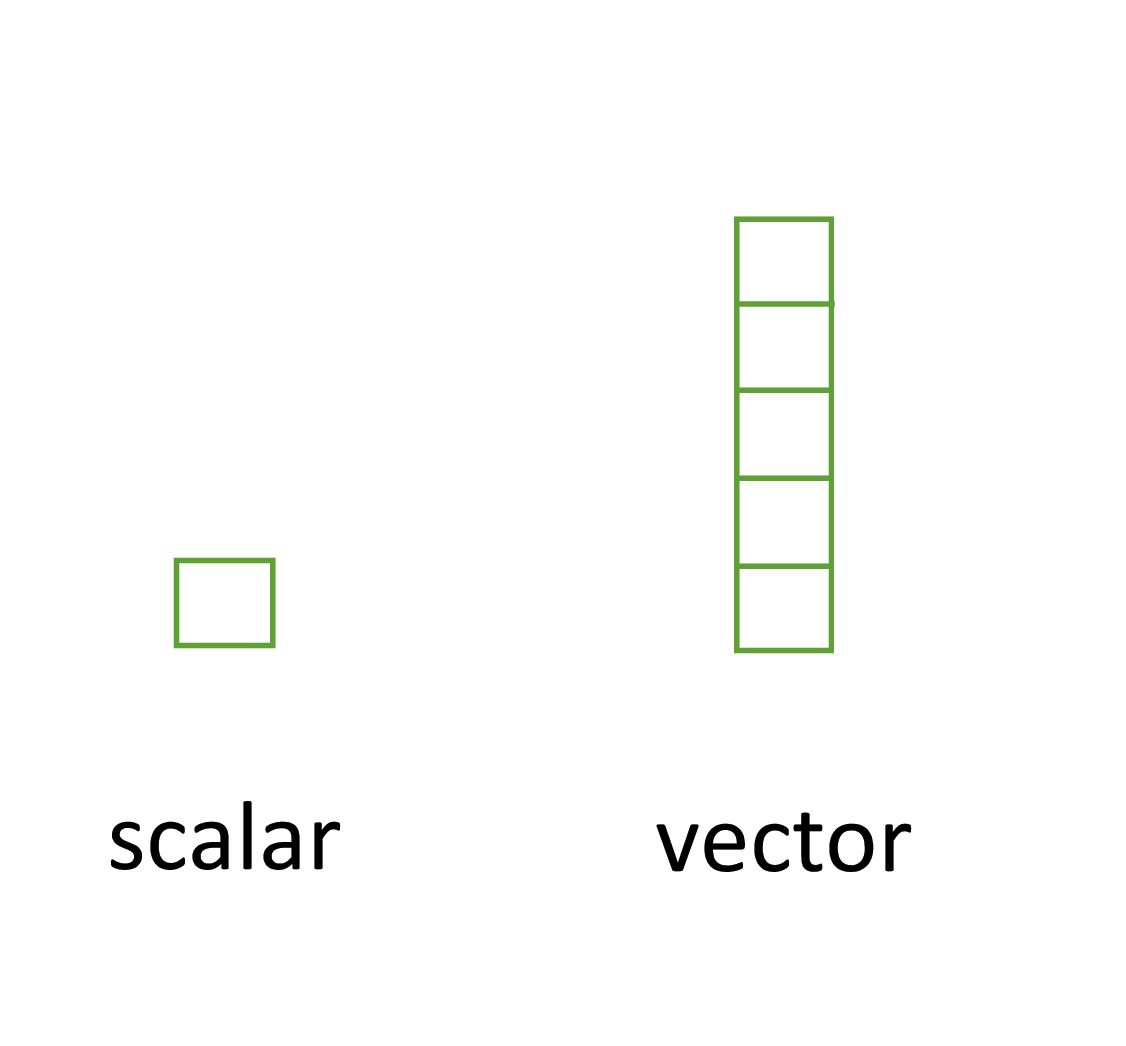
\includegraphics[width=\textwidth]{scal_vec}
\colc
\end{frame}



\bfr{Matrices and arrays}

\cola
\bi
\li A matrix is a vector with additional attributes called {\em dimensions}.
\li Arrays are multidimensional matrices.
\li Matrices and arrays can contain only a single type.
\li They may also contain NAs.
\ei
\colb
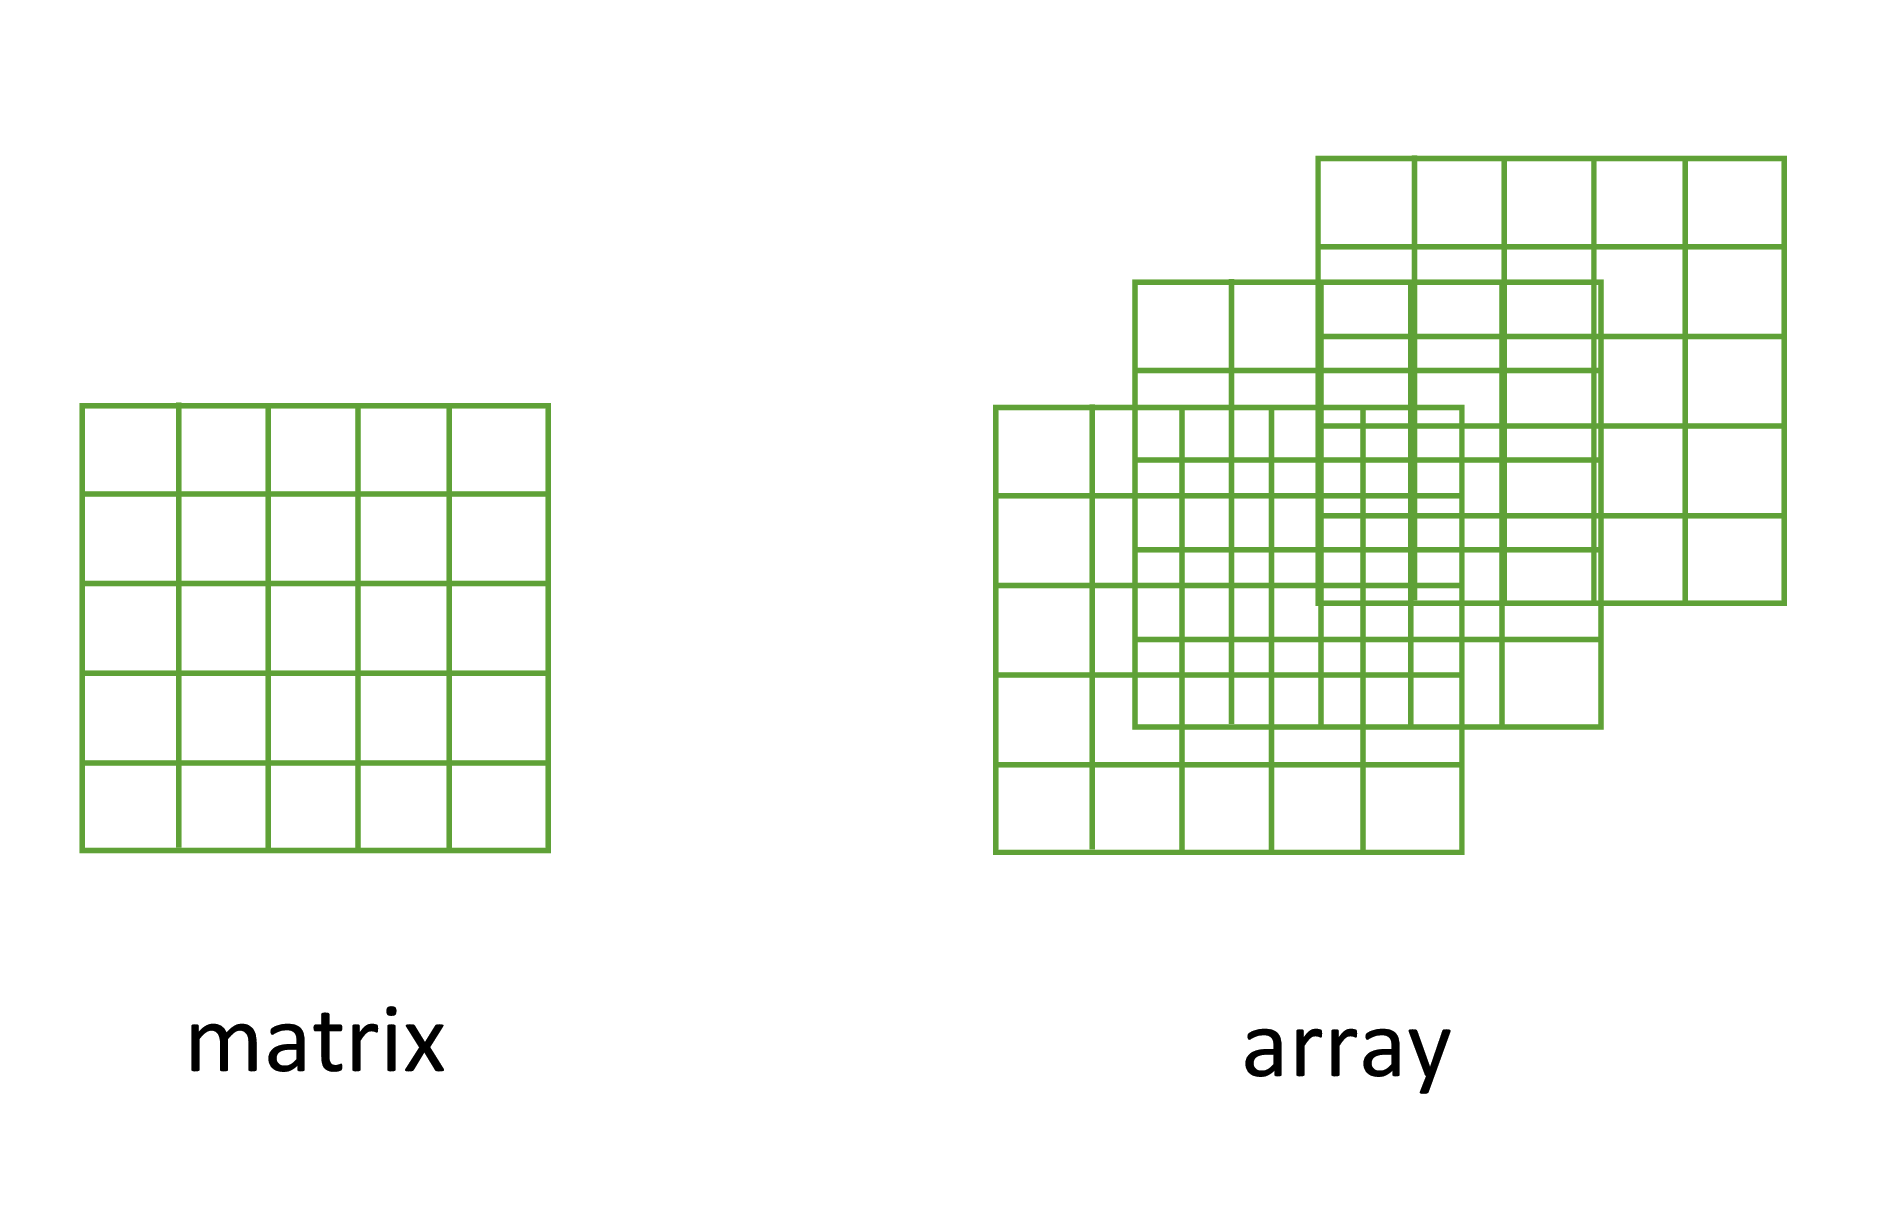
\includegraphics[width=\textwidth]{mat_array}
\colc
\end{frame}

\bfr{Creating matrices and arrays}
{\scriptsize
\begin{verbatim}
my_mat <- matrix(1:16, nrow = 4, byrow = TRUE)
my_mat
##      [,1] [,2] [,3] [,4]
## [1,]    1    2    3    4
## [2,]    5    6    7    8
## [3,]    9   10   11   12
## [4,]   13   14   15   16

my_array <- array(1:16, dim = c(2, 4, 2))
my_array
## , , 1
## 
##      [,1] [,2] [,3] [,4]
## [1,]    1    3    5    7
## [2,]    2    4    6    8
## 
## , , 2
## 
##      [,1] [,2] [,3] [,4]
## [1,]    9   11   13   15
## [2,]   10   12   14   16
\end{verbatim}
}
\end{frame}


\bfr{Optional row and column names}
\begin{verbatim}
rownames(my_mat) <- c("A", "B", "C", "D")
colnames(my_mat) <- c("a", "b", "c", "d")
my_mat
##    a  b  c  d
## A  1  2  3  4
## B  5  6  7  8
## C  9 10 11 12
## D 13 14 15 16
\end{verbatim}
\end{frame}


\bfr{Transpose a matrix}
\begin{verbatim}
my_mat_t <- t(my_mat)
my_mat_t
##   A B  C  D
## a 1 5  9 13
## b 2 6 10 14
## c 3 7 11 15
## d 4 8 12 16
\end{verbatim}
\end{frame}

\bfr{Diagonal elements}
\begin{verbatim}
my_mat_diag <- diag(my_mat)
my_mat_diag
## [1]  1  6 11 16
\end{verbatim}
\end{frame}

\bfr{Matrix arithmetic}
{\scriptsize
\begin{verbatim}
mat.1 <- matrix(c(2, 0, 1, 1), nrow = 2)   
                 # notice that the matrix has been filled 
                 # column-wise by default
mat.1                         
##      [,1] [,2]
## [1,]    2    1
## [2,]    0    1

mat.2 <- matrix(c(1, 1, 0, 2), nrow = 2)
mat.2
##      [,1] [,2]
## [1,]    1    0
## [2,]    1    2

mat.1 + mat.2           # matrix addition
##      [,1] [,2]
## [1,]    3    1
## [2,]    1    3
mat.1 * mat.2           # element by element products
##      [,1] [,2]
## [1,]    2    0
## [2,]    0    2
\end{verbatim}
}
\end{frame}

\bfr{Matrix multiplication }
\begin{verbatim}
mat.1 <- matrix(c(2, 0, 1, 1), nrow = 2)  
mat.1                         
##      [,1] [,2]
## [1,]    2    1
## [2,]    0    1

mat.2 <- matrix(c(1, 1, 0, 2), nrow = 2)
mat.2
##      [,1] [,2]
## [1,]    1    0
## [2,]    1    2


mat.1 %*% mat.2         # matrix multiplication
##      [,1] [,2]
## [1,]    3    2
## [2,]    1    2
\end{verbatim}
\end{frame}

\bfr{Lists}
\bi
\li Notice the double bracket [[ ]] for list items.
\ei
\begin{verbatim}
list_1 <- list(c("black", "yellow", "orange"),
               c(TRUE, TRUE, FALSE, TRUE, FALSE, FALSE),
               matrix(1:6, nrow = 3))
list_1
## [[1]]
## [1] "black"  "yellow" "orange"
## 
## [[2]]
## [1]  TRUE  TRUE FALSE  TRUE FALSE FALSE
## 
## [[3]]
##      [,1] [,2]
## [1,]    1    4
## [2,]    2    5
## [3,]    3    6
\end{verbatim}
\end{frame}

\bfr{List elements can be named}
\begin{verbatim}
list_2 <- list(colours = c("black", "yellow", "orange"), 
               evaluation = c(TRUE, TRUE ,FALSE, 
                              TRUE, FALSE, FALSE), 
               time = matrix(1:6, nrow = 3))
list_2
## $colours
## [1] "black"  "yellow" "orange"
## 
## $evaluation
## [1]  TRUE  TRUE FALSE  TRUE FALSE FALSE
## 
## $time
##      [,1] [,2]
## [1,]    1    4
## [2,]    2    5
## [3,]    3    6
\end{verbatim}
\end{frame}

\bfr{List elements can be renamed using \lst{names}}
\begin{verbatim}
names(list_1) <- c("colours", "evaluation", "time")
list_1
## $colours
## [1] "black"  "yellow" "orange"
## 
## $evaluation
## [1]  TRUE  TRUE FALSE  TRUE FALSE FALSE
## 
## $time
##      [,1] [,2]
## [1,]    1    4
## [2,]    2    5
## [3,]    3    6
\end{verbatim}
\end{frame}

\bfr{Data frames}
{\scriptsize
\begin{tabular}{llrrrrrr}
treat&	nitrogen&	block&	height&	weight&	leafarea&	shootarea&	flowers\\\hline
tip&	medium&	1&	7.5&	7.62&	11.7&	31.9&	1\\
tip&	medium&	1&	10.7&	12.14&	14.1&	46.0&	10\\
tip&	medium&	1&	11.2&	12.76&	7.1&	66.7&	10\\
tip&	medium&	1&	10.4&	8.78&	11.9&	20.3&	1\\
tip&	medium&	1&	10.4&	13.58&	14.5&	26.9&	4\\
tip&	medium&	1&	9.8&	10.08&	12.2&	72.7&	9\\
notip&	low&	2&	3.7&	8.10&	10.5&	60.5&	6\\
notip&	low&	2&	3.2&	7.45&	14.1&	38.1&	4\\
notip&	low&	2&	3.9&	9.19&	12.4&	52.6&	9\\
notip&	low&	2&	3.3&	8.92&	11.6&	55.2&	6\\
notip&	low&	2&	5.5&	8.44&	13.5&	77.6&	9\\
notip&	low&	2&	4.4&	10.60&	16.2&	63.3&	6\\
\end{tabular}
}
\bi
\li Most used data structure for real world data.
\li Each row contains an individual {\bf observation}.
\li Each column contains a measured {\bf variable}.
\li Each column is a vector of a single type.
\li Columns can be different types.
\ei
\end{frame}


\bfr{Data frames}
{\scriptsize
\begin{tabular}{llrrrrrr}
treat&	nitrogen&	block&	height&	weight&	leafarea&	shootarea&	flowers\\\hline
tip&	medium&	1&	7.5&	7.62&	11.7&	31.9&	1\\
tip&	medium&	1&	10.7&	12.14&	14.1&	46.0&	10\\
tip&	medium&	1&	11.2&	12.76&	7.1&	66.7&	10\\
tip&	medium&	1&	10.4&	8.78&	11.9&	20.3&	1\\
tip&	medium&	1&	10.4&	13.58&	14.5&	26.9&	4\\
tip&	medium&	1&	9.8&	10.08&	12.2&	72.7&	9\\
notip&	low&	2&	3.7&	8.10&	10.5&	60.5&	6\\
notip&	low&	2&	3.2&	7.45&	14.1&	38.1&	4\\
notip&	low&	2&	3.9&	9.19&	12.4&	52.6&	9\\
notip&	low&	2&	3.3&	8.92&	11.6&	55.2&	6\\
notip&	low&	2&	5.5&	8.44&	13.5&	77.6&	9\\
notip&	low&	2&	4.4&	10.60&	16.2&	63.3&	6\\
\end{tabular}
}
\bi
\li Each row is an individual petunia plant.
\li treat and nitrogen are {\bf categorical} variables (factors)
\li treat has 2 levels, tip and notip
\li nitrogen has 3 levels, low, medium, high
\li height, weight, leafarea, and shootarea are numeric
\li flowers is an integer
\li block uses integers, but should be treated as a factor
\ei
\end{frame}

\bfr{Data frames}
{\scriptsize
\begin{tabular}{llrrrrrr}
treat&	nitrogen&	block&	height&	weight&	leafarea&	shootarea&	flowers\\\hline
tip&	medium&	1&	7.5&	7.62&	11.7&	31.9&	1\\
tip&	medium&	1&	10.7&	12.14&	14.1&	46.0&	10\\
tip&	medium&	1&	11.2&	12.76&	7.1&	66.7&	10\\
tip&	medium&	1&	10.4&	8.78&	11.9&	20.3&	1\\
tip&	medium&	1&	10.4&	13.58&	14.5&	26.9&	4\\
tip&	medium&	1&	9.8&	10.08&	12.2&	72.7&	9\\
notip&	low&	2&	3.7&	8.10&	10.5&	60.5&	6\\
notip&	low&	2&	3.2&	7.45&	14.1&	38.1&	4\\
notip&	low&	2&	3.9&	9.19&	12.4&	52.6&	9\\
notip&	low&	2&	3.3&	8.92&	11.6&	55.2&	6\\
notip&	low&	2&	5.5&	8.44&	13.5&	77.6&	9\\
notip&	low&	2&	4.4&	10.60&	16.2&	63.3&	6\\
\end{tabular}
}
\bi
\li This type of data is known as {\bf rectangular} or {\bf tidy} data.
\li Each column must have the same number of observations.
\li Missing data must have NAs in their position.
\li Spreadsheets are often NOT tidy.
\ei

\end{frame}

\bfr{Constructing data frames}
{
\scriptsize
\begin{verbatim}
p.height <- c(180, 155, 160, 167, 181)
p.weight <- c(65, 50, 52, 58, 70)
p.names <- c("Joanna", "Charlotte", "Helen", "Karen", "Amy")

dataf <- data.frame(height = p.height, 
                    weight = p.weight, 
                    names = p.names)
dataf
##   height weight     names
## 1    180     65    Joanna
## 2    155     50 Charlotte
## 3    160     52     Helen
## 4    167     58     Karen
## 5    181     70       Amy

\end{verbatim}
}
\bi
\li Column names are taken from the constructor.
\li Can be changed with \lst{names}.
\li Numbers at left are row names automatically produced by R, not another column.
\li If the vectors are not the same length R will (quietly) cycle!
\ei
\end{frame}



\bfr{Structure of  data frames}
\begin{verbatim}
dim(dataf)   # 5 rows and 3 columns
## [1] 5 3

str(dataf)   
## 'data.frame':    5 obs. of  3 variables:
##  $ height: num  180 155 160 167 181
##  $ weight: num  65 50 52 58 70
##  $ names : chr  "Joanna" "Charlotte" "Helen" "Karen" ...
\end{verbatim}
\bi
\li Gives type, dimensions, column names, types, a few values.
\li Convenient to place this in a comment block in your code when
dealing with a data frame, for reference.
\li R has automatically made names a character vector, not a factor.
\ei
\end{frame}

\bfr{Automatically convert strings to factors}
\scriptsize
\begin{verbatim}
p.height <- c(180, 155, 160, 167, 181)
p.weight <- c(65, 50, 52, 58, 70)
p.names <- c("Joanna", "Charlotte", "Helen", "Karen", "Amy")

dataf <- data.frame(height = p.height, 
                    weight = p.weight,
                    names = p.names, 
                    stringsAsFactors = TRUE)
str(dataf)
## 'data.frame':    5 obs. of  3 variables:
##  $ height: num  180 155 160 167 181
##  $ weight: num  65 50 52 58 70
##  $ names : Factor w/ 5 levels "Amy","Charlotte",..: 4 2 3 5 1
\end{verbatim}


\end{frame}

\bfr{Preparing data for import}
\cola
\bi
\li Easiest way to enter data is use Excel or LibreOffice Calc.
\li Save data in tab-delimited or comma-delimited file.
\li Keep column headings short.
\li No spaces in column headings.
\li Avoid special characters, e.g., \verb|mm^2|
\li No empty cells!  Use NAs.
\li Make sure it's tidy!
\ei
\colb
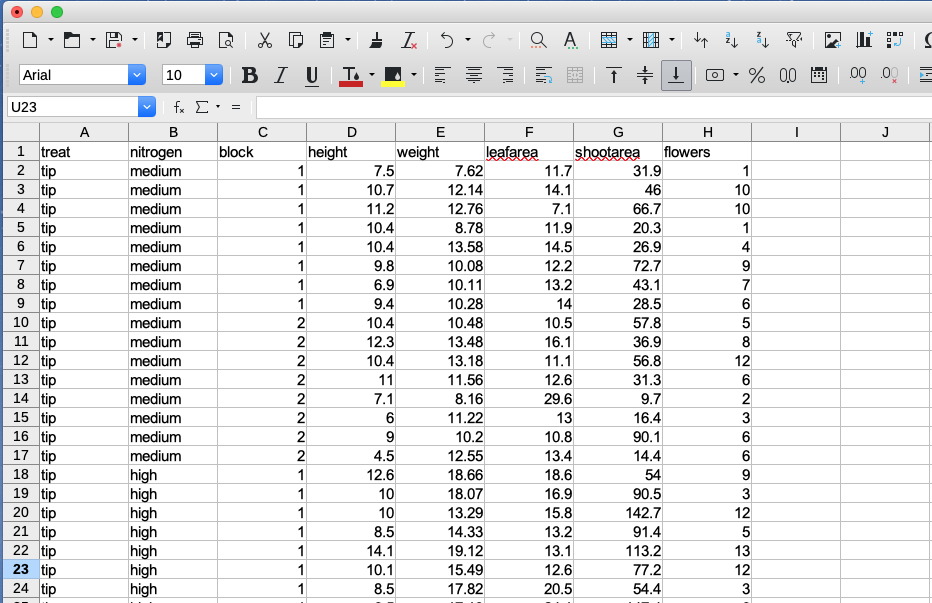
\includegraphics[width=\textwidth]{libre_off}
\colc

\vfill

\bi
\li {\bf Beware!} \url{https://genomebiology.biomedcentral.com/articles/10.1186/s13059-016-1044-7}
\ei
\end{frame}

\bfr{Importing}
\begin{verbatim}
flowers <- read.table(file = 'data/flower.txt',
                      header = TRUE, sep = "\t",
                      stringsAsFactors = TRUE)
\end{verbatim}

\bi
\li Forward slash works on ALL systems.
\li \verb|header=TRUE| means the first line is variable names.
\li \verb|sep="\t"| for tab-delimited files
\li \verb|sep=","| for comma-delimited files
\ei
\end{frame}


\bfr{Importing}
\begin{verbatim}
> str(flowers) 
'data.frame':    96 obs. of  8 variables:
  $ treat    : Factor w/ 2 levels "notip","tip": 2 2 2 2 2 2 2 2 2 2 ...
  $ nitrogen : Factor w/ 3 levels "high","low","medium": 3 3 3 3 3 3 3 3 3 3 ...
  $ block    : int  1 1 1 1 1 1 1 1 2 2 ...
  $ height   : num  7.5 10.7 11.2 10.4 10.4 9.8 6.9 9.4 10.4 12.3 ...
  $ weight   : num  7.62 12.14 12.76 8.78 13.58 ...
  $ leafarea : num  11.7 14.1 7.1 11.9 14.5 12.2 13.2 14 10.5 16.1 ...
  $ shootarea: num  31.9 46 66.7 20.3 26.9 72.7 43.1 28.5 57.8 36.9 ...
  $ flowers  : int  1 10 10 1 4 9 7 6 5 8 .
\end{verbatim}

\bi
\li After importing check structure of data frame.
\li treat and nitrogen have been converted to factors.
\li Usually very helpful to include this as a comment block in your script.
\ei
\end{frame}

\bfr{Specialized import functions}
\begin{verbatim}
# import .csv file with sep = "\t" and header = FALSE
flowers <- read.table(file = 'data/flower.txt') 

# import .csv file with sep = "," 
# and header = TRUE
flowers <- read.csv(file = 'data/flower.csv') 

# import .csv file with dec = "," and sep = ";" 
# and header = TRUE
flowers <- read.csv2(file = 'data/flower.csv') 

# import tab delim file with sep = "\t" and header = TRUE
flowers <- read.delim(file = 'data/flower.txt') 
\end{verbatim}

\bi
\li Avoid importing from spreadsheet files (\verb|.xls| {\em etc.}).
\ei
\end{frame}


\bfr{Import problems}
\begin{verbatim}
Error in file(file, "rt") : cannot open the connection
In addition: Warning message:
In file(file, "rt") :
  cannot open file 'flower.txt': No such file or directory
\end{verbatim}
\bi
\li Spelling mistakes.
\li Wrong working directory.
\li Forgot the extension (\verb|.txt|, \verb|.csv|, {\em etc.}).
\ei
\end{frame}

\bfr{Forgot {\tt header = TRUE}}
\begin{verbatim}
flowers_bad <- read.table(file = 'data/flower.txt',
                          sep = "\t")
str(flowers_bad)
## 'data.frame':    97 obs. of  8 variables:
##  $ V1: chr  "treat" "tip" "tip" "tip" ...
##  $ V2: chr  "nitrogen" "medium" "medium" "medium" ...
##  $ V3: chr  "block" "1" "1" "1" ...
##  $ V4: chr  "height" "7.5" "10.7" "11.2" ...
##  $ V5: chr  "weight" "7.62" "12.14" "12.76" ...
##  $ V6: chr  "leafarea" "11.7" "14.1" "7.1" ...
##  $ V7: chr  "shootarea" "31.9" "46" "66.7" ...
##  $ V8: chr  "flowers" "1" "10" "10" ...
\end{verbatim}
\bi
\li All of our variables are character (or factor).
\li The first value of each variable is the column name.
\li R has provided default names, \verb|V1, V2, V3, ...|
\ei
\end{frame}

\bfr{Alternative loader functions}
\begin{verbatim}
library(readr)
# import white space delimited files
all_data <- read_table(file = 'data/flower.txt',
                       col_names = TRUE)

# import comma delimited files
all_data <- read_csv(file = 'data/flower.txt')

# import tab delimited files
all_data <- read_delim(file = 'data/flower.txt', 
                       delim = "\t")

# or use
all_data <- read_tsv(file = 'data/flower.txt')
\end{verbatim}
\bi
\li \verb|readr| is from the {\bf tidyverse} collection of packages.
\li Many of the arguments are the same as \verb|read.table|
\li Returns a \verb|tibble|, which is very similar to a data frame.
\ei

\end{frame}

\bfr{Packages for large datasets}
\bi
\li \verb|read.table|
\li \verb|ff|
\li \verb|bigmemory|
\ei

\end{frame}

\bfr{Do exercise 3, part 1}
\end{frame}

\bfr{Wrangling data frames}
\begin{verbatim}
flowers <- read.table(file = 'data/flower.txt', header = TRUE, sep = "\t")
str(flowers)
## 'data.frame':    96 obs. of  8 variables:
##  $ treat    : chr  "tip" "tip" "tip" "tip" ...
##  $ nitrogen : chr  "medium" "medium" "medium" "medium" ...
##  $ block    : int  1 1 1 1 1 1 1 1 2 2 ...
##  $ height   : num  7.5 10.7 11.2 10.4 10.4 9.8 6.9 9.4 10.4 12.3 ...
##  $ weight   : num  7.62 12.14 12.76 8.78 13.58 ...
##  $ leafarea : num  11.7 14.1 7.1 11.9 14.5 12.2 13.2 14 10.5 16.1 ...
##  $ shootarea: num  31.9 46 66.7 20.3 26.9 72.7 43.1 28.5 57.8 36.9 ...
##  $ flowers  : int  1 10 10 1 4 9 7 6 5 8 ...
\end{verbatim}

\end{frame}

\bfr{The \$ notation}
\scriptsize
\begin{verbatim}
flowers$height
 [1]  7.5 10.7 11.2 10.4 10.4  9.8  6.9  9.4 10.4 12.3 10.4
[12] 11.0  7.1  6.0  9.0  4.5 12.6 10.0 10.0  8.5 14.1 10.1
[23]  8.5  6.5 11.5  7.7  6.4  8.8  9.2  6.2  6.3 17.2  8.0
[34]  8.0  6.4  7.6  9.7 12.3  9.1  8.9  7.4  3.1  7.9  8.8
[45]  8.5  5.6 11.5  5.8  5.6  5.3  7.5  4.1  3.5  8.5  4.9
[56]  2.5  5.4  3.9  5.8  4.5  8.0  1.8  2.2  3.9  8.5  8.5
[67]  6.4  1.2  2.6 10.9  7.2  2.1  4.7  5.0  6.5  2.6  6.0
[78]  9.3  4.6  5.2  3.9  2.3  5.2  2.2  4.5  1.8  3.0  3.7
[89]  2.4  5.7  3.7  3.2  3.9  3.3  5.5  4.4

f_height <- flowers$height
mean(f_height)
## [1] 6.839583
summary(f_height)
##    Min. 1st Qu.  Median    Mean 3rd Qu.    Max. 
##   1.200   4.475   6.450   6.840   9.025  17.200

mean(flowers$height)
## [1] 6.839583
summary(flowers$height)
##    Min. 1st Qu.  Median    Mean 3rd Qu.    Max. 
##   1.200   4.475   6.450   6.840   9.025  17.200
\end{verbatim}

\end{frame}

\bfr{Positional indexes}

\begin{verbatim}
flowers[1, 4]
## [1] 7.5

# this would give you the same
flowers$height[1]
## [1] 7.5
\end{verbatim}

\end{frame}

\bfr{Positional indexes}

\begin{verbatim}
flowers[1:10, 1:4]
##    treat nitrogen block height
## 1    tip   medium     1    7.5
## 2    tip   medium     1   10.7
## 3    tip   medium     1   11.2
## 4    tip   medium     1   10.4
## 5    tip   medium     1   10.4
## 6    tip   medium     1    9.8
## 7    tip   medium     1    6.9
## 8    tip   medium     1    9.4
## 9    tip   medium     2   10.4
## 10   tip   medium     2   12.3
\end{verbatim}

\end{frame}

\bfr{Positional indexes}

\begin{verbatim}
flowers[c(1, 5, 12, 30), c(1, 3, 6, 8)]
##    treat block leafarea flowers
## 1    tip     1     11.7       1
## 5    tip     1     14.5       4
## 12   tip     2     12.6       6
## 30   tip     2     11.6       5
\end{verbatim}

\end{frame}

\bfr{Empty index means "all of them"}

\begin{verbatim}
flowers[1:8, ]
##   treat nitrogen block height weight leafarea shootarea flowers
## 1   tip   medium     1    7.5   7.62     11.7      31.9       1
## 2   tip   medium     1   10.7  12.14     14.1      46.0      10
## 3   tip   medium     1   11.2  12.76      7.1      66.7      10
## 4   tip   medium     1   10.4   8.78     11.9      20.3       1
## 5   tip   medium     1   10.4  13.58     14.5      26.9       4
## 6   tip   medium     1    9.8  10.08     12.2      72.7       9
## 7   tip   medium     1    6.9  10.11     13.2      43.1       7
## 8   tip   medium     1    9.4  10.28     14.0      28.5       6
\end{verbatim}

\end{frame}

\bfr{Negative numbers mean "not these"}

\begin{verbatim}
flowers[-(1:85), -c(4, 7, 8)]
##    treat nitrogen block weight leafarea
## 86 notip      low     1   6.01     17.6
## 87 notip      low     1   9.93     12.0
## 88 notip      low     1   7.03      7.9
## 89 notip      low     2   9.10     14.5
## 90 notip      low     2   9.05      9.6
## 91 notip      low     2   8.10     10.5
## 92 notip      low     2   7.45     14.1
## 93 notip      low     2   9.19     12.4
## 94 notip      low     2   8.92     11.6
## 95 notip      low     2   8.44     13.5
## 96 notip      low     2  10.60     16.2
\end{verbatim}

\end{frame}

\bfr{Can also use column names}

\begin{verbatim}
flowers[1:5, c("treat", "nitrogen", "leafarea")]
##   treat nitrogen leafarea
## 1   tip   medium     11.7
## 2   tip   medium     14.1
## 3   tip   medium      7.1
## 4   tip   medium     11.9
## 5   tip   medium     14.5
\end{verbatim}

\bi
\li More readable and portable than \verb|flowers[1:5, c(1, 2, 6)]|
\ei

\end{frame}


\bfr{Logical indexes}

\begin{verbatim}
big_flowers <- flowers[flowers$height > 12, ]
big_flowers
##    treat nitrogen block height weight leafarea shootarea flowers
## 10   tip   medium     2   12.3  13.48     16.1      36.9       8
## 17   tip     high     1   12.6  18.66     18.6      54.0       9
## 21   tip     high     1   14.1  19.12     13.1     113.2      13
## 32   tip     high     2   17.2  19.20     10.9      89.9      14
## 38   tip      low     1   12.3  11.27     13.7      28.7       5
\end{verbatim}


\end{frame}



\bfr{Logical indexes}

\begin{verbatim}
nit_high <- flowers[flowers$nitrogen == "high", ]        
nit_high
##    treat nitrogen block height weight leafarea shootarea flowers
## 17   tip     high     1   12.6  18.66     18.6      54.0       9
## 18   tip     high     1   10.0  18.07     16.9      90.5       3
## 19   tip     high     1   10.0  13.29     15.8     142.7      12
## 20   tip     high     1    8.5  14.33     13.2      91.4       5
## 21   tip     high     1   14.1  19.12     13.1     113.2      13
## 22   tip     high     1   10.1  15.49     12.6      77.2      12
....
\end{verbatim}


\end{frame}


\bfr{Logical indexes}

\begin{verbatim}
low_notip_high6 <- flowers[flowers$height >= 6 & 
                           flowers$nitrogen == "medium" &
                           flowers$treat == "notip", ]        
low_notip_high6
##    treat nitrogen block height weight leafarea shootarea flowers
## 51 notip   medium     1    7.5  13.60     13.6     122.2      11
## 54 notip   medium     1    8.5  10.04     12.3     113.6       4
## 61 notip   medium     2    8.0  11.43     12.6      43.2      14
\end{verbatim}


\end{frame}


\bfr{Vectorized and nonvectorized logical operators}
\begin{verbatim}
> x <- c(T,T,F,F)
> y <- c(T,F,T,F)
> x | y
[1]  TRUE  TRUE  TRUE FALSE
> x || y
[1] TRUE
> x & y
[1]  TRUE FALSE FALSE FALSE
> x && y
[1] TRUE
\end{verbatim}
\end{frame}

\bfr{Logical indexes using {\tt subset}}

\begin{verbatim}
tip_med_2 <- subset(flowers, treat == "tip" &
                    nitrogen == "medium" & 
                    block == 2)
tip_med_2
##    treat nitrogen block height weight leafarea shootarea flowers
## 9    tip   medium     2   10.4  10.48     10.5      57.8       5
## 10   tip   medium     2   12.3  13.48     16.1      36.9       8
## 11   tip   medium     2   10.4  13.18     11.1      56.8      12
## 12   tip   medium     2   11.0  11.56     12.6      31.3       6
## 13   tip   medium     2    7.1   8.16     29.6       9.7       2
## 14   tip   medium     2    6.0  11.22     13.0      16.4       3
## 15   tip   medium     2    9.0  10.20     10.8      90.1       6
## 16   tip   medium     2    4.5  12.55     13.4      14.4       6
\end{verbatim}
\bi
\li We don't need to use \verb|flowers$treat|
\ei

\end{frame}

\bfr{Logical indexes using {\tt subset} and {\tt select}}

\begin{verbatim}
tipplants <- subset(flowers,
               treat == "tip" &  
               nitrogen == "medium" & 
               block == 2, 
               select = c("treat", "nitrogen", "leafarea"))
tipplants
##    treat nitrogen leafarea
## 9    tip   medium     10.5
## 10   tip   medium     16.1
## 11   tip   medium     11.1
## 12   tip   medium     12.6
## 13   tip   medium     29.6
## 14   tip   medium     13.0
## 15   tip   medium     10.8
## 16   tip   medium     13.4
\end{verbatim}
\bi
\li Selecting both rows and columns.
\ei

\end{frame}

\bfr{Ordering data frames}
\begin{verbatim}
height_ord <- flowers[order(flowers$height), ]        
height_ord
##    treat nitrogen block height weight leafarea shootarea flowers
## 68 notip     high     1    1.2  18.24     16.6     148.1       7
## 62 notip   medium     2    1.8  10.47     11.8     120.8       9
## 86 notip      low     1    1.8   6.01     17.6      46.2       4
## 72 notip     high     1    2.1  19.15     15.6     176.7       6
## 63 notip   medium     2    2.2  10.70     15.3      97.1       7
## 84 notip      low     1    2.2   9.97      9.6      63.1       2
## 82 notip      low     1    2.3   7.28     13.8      32.8       6
## 89 notip      low     2    2.4   9.10     14.5      78.7       8
## 56 notip   medium     1    2.5  14.85     17.5      77.8      10
## 69 notip     high     1    2.6  16.57     17.1     141.1       3
## 76 notip     high     2    2.6  18.88     16.4     181.5      14
## 87 notip      low     1    3.0   9.93     12.0      56.6       6
## 42   tip      low     2    3.1   8.74     16.1      39.1       3
...
\end{verbatim}
\end{frame}


\bfr{Ordering data frames}
\begin{verbatim}
leafarea_ord <- flowers[order(flowers$leafarea, decreasing = TRUE), ]        
leafarea_ord
##    treat nitrogen block height weight leafarea shootarea flowers
## 70 notip     high     1   10.9  17.22     49.2     189.6      17
## 13   tip   medium     2    7.1   8.16     29.6       9.7       2
## 24   tip     high     1    6.5  17.13     24.1     147.4       6
## 65 notip     high     1    8.5  22.53     20.8     166.9      16
## 23   tip     high     1    8.5  17.82     20.5      54.4       3
## 66 notip     high     1    8.5  17.33     19.8     184.4      12
## 73 notip     high     2    4.7  13.42     19.8     124.7       5
## 80 notip     high     2    5.2  17.70     19.1     181.1       8
## 17   tip     high     1   12.6  18.66     18.6      54.0       9
## 49 notip   medium     1    5.6  11.03     18.6      49.9       8
## 78 notip     high     2    9.3  18.75     18.4     181.1      16
...
\end{verbatim}
\end{frame}



\bfr{Ordering data frames}
\scriptsize
\begin{verbatim}
block_height_ord <- flowers[order(flowers$block, flowers$height), ]        
block_height_ord
##    treat nitrogen block height weight leafarea shootarea flowers
## 68 notip     high     1    1.2  18.24     16.6     148.1       7
## 86 notip      low     1    1.8   6.01     17.6      46.2       4
## 72 notip     high     1    2.1  19.15     15.6     176.7       6
## 84 notip      low     1    2.2   9.97      9.6      63.1       2
## 82 notip      low     1    2.3   7.28     13.8      32.8       6
## 56 notip   medium     1    2.5  14.85     17.5      77.8      10
## 69 notip     high     1    2.6  16.57     17.1     141.1       3
....
## 38   tip      low     1   12.3  11.27     13.7      28.7       5
## 17   tip     high     1   12.6  18.66     18.6      54.0       9
## 21   tip     high     1   14.1  19.12     13.1     113.2      13
## 62 notip   medium     2    1.8  10.47     11.8     120.8       9
## 63 notip   medium     2    2.2  10.70     15.3      97.1       7
## 89 notip      low     2    2.4   9.10     14.5      78.7       8
## 76 notip     high     2    2.6  18.88     16.4     181.5      14
## 42   tip      low     2    3.1   8.74     16.1      39.1       3
## 92 notip      low     2    3.2   7.45     14.1      38.1       4
....
\end{verbatim}
\end{frame}




\bfr{Ordering data frames}
\scriptsize
\begin{verbatim}
block_revheight_ord <- flowers[order(flowers$block, -flowers$height), ]        
block_revheight_ord
##    treat nitrogen block height weight leafarea shootarea flowers
## 21   tip     high     1   14.1  19.12     13.1     113.2      13
## 17   tip     high     1   12.6  18.66     18.6      54.0       9
## 38   tip      low     1   12.3  11.27     13.7      28.7       5
## 3    tip   medium     1   11.2  12.76      7.1      66.7      10
## 70 notip     high     1   10.9  17.22     49.2     189.6      17
## 2    tip   medium     1   10.7  12.14     14.1      46.0      10
## 4    tip   medium     1   10.4   8.78     11.9      20.3       1
## 5    tip   medium     1   10.4  13.58     14.5      26.9       4
## 22   tip     high     1   10.1  15.49     12.6      77.2      12
....
## 72 notip     high     1    2.1  19.15     15.6     176.7       6
## 86 notip      low     1    1.8   6.01     17.6      46.2       4
## 68 notip     high     1    1.2  18.24     16.6     148.1       7
## 32   tip     high     2   17.2  19.20     10.9      89.9      14
## 10   tip   medium     2   12.3  13.48     16.1      36.9       8
## 25   tip     high     2   11.5  23.89     14.3     101.5      12
## 47   tip      low     2   11.5   8.72     10.2      28.3       6
## 12   tip   medium     2   11.0  11.56     12.6      31.3       6
....
\end{verbatim}
\end{frame}



\bfr{Ordering data frames}
\scriptsize
\begin{verbatim}
revheight_ord <- flowers[order(-xtfrm(flowers$nitrogen), flowers$height), ]        
revheight_ord
##    treat nitrogen block height weight leafarea shootarea flowers
## 62 notip   medium     2    1.8  10.47     11.8     120.8       9
## 63 notip   medium     2    2.2  10.70     15.3      97.1       7
## 56 notip   medium     1    2.5  14.85     17.5      77.8      10
## 53 notip   medium     1    3.5  12.93     16.6     109.3       3
## 58 notip   medium     2    3.9   9.07      9.6      90.4       7
....
## 2    tip   medium     1   10.7  12.14     14.1      46.0      10
## 12   tip   medium     2   11.0  11.56     12.6      31.3       6
## 3    tip   medium     1   11.2  12.76      7.1      66.7      10
## 10   tip   medium     2   12.3  13.48     16.1      36.9       8
## 86 notip      low     1    1.8   6.01     17.6      46.2       4
## 84 notip      low     1    2.2   9.97      9.6      63.1       2
....
## 39   tip      low     1    9.1   8.96      9.7      23.8       3
## 37   tip      low     1    9.7   6.49      8.1      18.0       3
## 47   tip      low     2   11.5   8.72     10.2      28.3       6
## 38   tip      low     1   12.3  11.27     13.7      28.7       5
## 68 notip     high     1    1.2  18.24     16.6     148.1       7
## 72 notip     high     1    2.1  19.15     15.6     176.7       6
## 69 notip     high     1    2.6  16.57     17.1     141.1       3
....
\end{verbatim}
\end{frame}


\bfr{Ordering data frames}
\scriptsize
\begin{verbatim}
flowers$nitrogen <- factor(flowers$nitrogen, 
                           levels = c("low", "medium", "high"))    
nit_ord <- flowers[order(flowers$nitrogen),]
nit_ord
##    treat nitrogen block height weight leafarea shootarea flowers
## 33   tip      low     1    8.0   6.88      9.3      16.1       4
## 34   tip      low     1    8.0  10.23     11.9      88.1       4
## 35   tip      low     1    6.4   5.97      8.7       7.3       2
## 36   tip      low     1    7.6  13.05      7.2      47.2       8
....
## 94 notip      low     2    3.3   8.92     11.6      55.2       6
## 95 notip      low     2    5.5   8.44     13.5      77.6       9
## 96 notip      low     2    4.4  10.60     16.2      63.3       6
## 1    tip   medium     1    7.5   7.62     11.7      31.9       1
## 2    tip   medium     1   10.7  12.14     14.1      46.0      10
## 3    tip   medium     1   11.2  12.76      7.1      66.7      10
....
## 62 notip   medium     2    1.8  10.47     11.8     120.8       9
## 63 notip   medium     2    2.2  10.70     15.3      97.1       7
## 64 notip   medium     2    3.9  12.97     17.0      97.5       5
## 17   tip     high     1   12.6  18.66     18.6      54.0       9
## 18   tip     high     1   10.0  18.07     16.9      90.5       3
## 19   tip     high     1   10.0  13.29     15.8     142.7      12
....
\end{verbatim}
\end{frame}

\bfr{Adding rows to a data frame}
\begin{verbatim}
# rbind for rows
df1 <- data.frame(id = 1:4, height = c(120, 150, 132, 122),
                        weight = c(44, 56, 49, 45))
df1
##   id height weight
## 1  1    120     44
## 2  2    150     56
## 3  3    132     49
## 4  4    122     45

df2 <- data.frame(id = 5:6, height = c(119, 110),
                        weight = c(39, 35))
df2
##   id height weight
## 1  5    119     39
## 2  6    110     35
\end{verbatim}
\end{frame}

\bfr{Adding rows to a data frame}
\begin{verbatim}
df_rcomb <- rbind(df1, df2)
df_rcomb
##   id height weight
## 1  1    120     44
## 2  2    150     56
## 3  3    132     49
## 4  4    122     45
## 5  5    119     39
## 6  6    110     35
\end{verbatim}
\end{frame}


\bfr{Adding columns to a data frame}
\begin{verbatim}
df3 <- data.frame(id = 1:4, height = c(120, 150, 132, 122),
                        weight = c(44, 56, 49, 45))
df3
##   id height weight
## 1  1    120     44
## 2  2    150     56
## 3  3    132     49
## 4  4    122     45

df4 <- data.frame(location = c("UK", "CZ", "CZ", "UK"))
df4
##   location
## 1       UK
## 2       CZ
## 3       CZ
## 4       UK
\end{verbatim}
\end{frame}


\bfr{Adding columns to a data frame}
\begin{verbatim}
df_ccomb <- cbind(df3, df4)
df_ccomb
##   id height weight location
## 1  1    120     44       UK
## 2  2    150     56       CZ
## 3  3    132     49       CZ
## 4  4    122     45       UK
\end{verbatim}
\end{frame}

\bfr{Adding computed columns to a data frame}
\begin{verbatim}
df_rcomb$height_log10 <- log10(df_rcomb$height)
df_rcomb
##   id height weight height_log10
## 1  1    120     44     2.079181
## 2  2    150     56     2.176091
## 3  3    132     49     2.120574
## 4  4    122     45     2.086360
## 5  5    119     39     2.075547
## 6  6    110     35     2.041393
\end{verbatim}
\end{frame}

\bfr{Converting type of a column}
\begin{verbatim}
# convert to a factor 
df_rcomb$Fid <- factor(df_rcomb$id)
df_rcomb
##   id height weight height_log10 Fid
## 1  1    120     44     2.079181   1
## 2  2    150     56     2.176091   2
## 3  3    132     49     2.120574   3
## 4  4    122     45     2.086360   4
## 5  5    119     39     2.075547   5
## 6  6    110     35     2.041393   6
str(df_rcomb)
## 'data.frame':    6 obs. of  5 variables:
##  $ id          : int  1 2 3 4 5 6
##  $ height      : num  120 150 132 122 119 110
##  $ weight      : num  44 56 49 45 39 35
##  $ height_log10: num  2.08 2.18 2.12 2.09 2.08 ...
##  $ Fid         : Factor w/ 6 levels "1","2","3","4",..: 1 2 3 4 5 6
\end{verbatim}
\end{frame}


\bfr{Merging data frames}
\bi
\li Suppose we have one data frame with information about some
common rocky shore invertebrates, called \verb|taxa|
\li And we have another data frame with infromation about where these invertebrates are usually found,
called \verb|zone|
\li Can we combine these into one data frame with all information about the invertebrates?
\ei
\end{frame}

\bfr{Merging data frames}
\scriptsize
\begin{verbatim}
taxa <- data.frame(
         GENUS = c("Patella", "Littorina", "Halichondria", "Semibalanus"),
         species = c("vulgata", "littoria", "panacea", "balanoides"),
         family = c("patellidae", "Littorinidae", "Halichondriidae", "Archaeobalanidae"))
taxa
##          GENUS    species           family
## 1      Patella    vulgata       patellidae
## 2    Littorina   littoria     Littorinidae
## 3 Halichondria    panacea  Halichondriidae
## 4  Semibalanus balanoides Archaeobalanidae

zone <- data.frame(
    genus = c("Laminaria", "Halichondria", "Xanthoria", "Littorina", "Semibalanus", "Fucus"),
    species = c("digitata", "panacea", "parietina", "littoria",    "balanoides", "serratus"),
    zone = c( "v_low", "low", "v_high", "low_mid", "high", "low_mid"))
zone
##          genus    species    zone
## 1    Laminaria   digitata   v_low
## 2 Halichondria    panacea     low
## 3    Xanthoria  parietina  v_high
## 4    Littorina   littoria low_mid
## 5  Semibalanus balanoides    high
## 6        Fucus   serratus low_mid
\end{verbatim}
\end{frame}

\bfr{Merging data frames}
{
\scriptsize
\begin{verbatim}
taxa_zone <- merge(x = taxa, y = zone)
taxa_zone
##      species        GENUS           family        genus    zone
## 1 balanoides  Semibalanus Archaeobalanidae  Semibalanus    high
## 2   littoria    Littorina     Littorinidae    Littorina low_mid
## 3    panacea Halichondria  Halichondriidae Halichondria     low
\end{verbatim}
}
\bi
\li Because the two data frames have a column name in common,
R assumes you want to join on that column.
\li The joined data frame has both \verb|GENUS| and \verb|genus| because
they are spelled differently.
\li The joined data frame has only those rows with information in BOTH
original data frames.
\ei
\end{frame}


\bfr{Merging data frames}
{
\scriptsize
\begin{verbatim}
taxa_zone <- merge(x = taxa, y = zone, all = TRUE)
taxa_zone
##      species        GENUS           family        genus    zone
## 1 balanoides  Semibalanus Archaeobalanidae  Semibalanus    high
## 2   digitata         <NA>             <NA>    Laminaria   v_low
## 3   littoria    Littorina     Littorinidae    Littorina low_mid
## 4    panacea Halichondria  Halichondriidae Halichondria     low
## 5  parietina         <NA>             <NA>    Xanthoria  v_high
## 6   serratus         <NA>             <NA>        Fucus low_mid
## 7    vulgata      Patella       patellidae         <NA>    <NA>
\end{verbatim}
}
\bi
\li To include ALL data from BOTH frames use \verb|all = TRUE|
\li NAs will be substituted for missing data.
\ei
\end{frame}



\bfr{Merging data frames}
\bi
\li Use \verb|by.x| and \verb|by.y| if the names are different
\ei
\scriptsize
\begin{verbatim}
taxa_zone <- merge(x = taxa, y = zone, 
                   by.x = "GENUS", 
                   by.y = "genus",
                   all = TRUE)
taxa_zone
##          GENUS  species.x           family  species.y    zone
## 1        Fucus       <NA>             <NA>   serratus low_mid
## 2 Halichondria    panacea  Halichondriidae    panacea     low
## 3    Laminaria       <NA>             <NA>   digitata   v_low
## 4    Littorina   littoria     Littorinidae   littoria low_mid
## 5      Patella    vulgata       patellidae       <NA>    <NA>
## 6  Semibalanus balanoides Archaeobalanidae balanoides    high
## 7    Xanthoria       <NA>             <NA>  parietina  v_high
\end{verbatim}

\end{frame}

\bfr{Merging data frames}
\bi
\li Can use multiple columns
\ei
\begin{verbatim}
taxa_zone <- merge(x = taxa, y = zone, 
                   by.x = c("species", "GENUS"), 
                   by.y = c("species", "genus"), 
                   all = TRUE)
taxa_zone
##      species        GENUS           family    zone
## 1 balanoides  Semibalanus Archaeobalanidae    high
## 2   digitata    Laminaria             <NA>   v_low
## 3   littoria    Littorina     Littorinidae low_mid
## 4    panacea Halichondria  Halichondriidae     low
## 5  parietina    Xanthoria             <NA>  v_high
## 6   serratus        Fucus             <NA> low_mid
## 7    vulgata      Patella       patellidae    <NA>
\end{verbatim}

\end{frame}

\bfr{Reshaping data frames}
\scriptsize
\begin{verbatim}
long_data <- data.frame(
   subject = rep(c("A", "B", "C", "D"), each = 3),
   sex = rep(c("M", "F", "F", "M"), each =3),
   condition = rep(c("control", "cond1", "cond2"), times = 4),
   measurement = c(12.9, 14.2, 8.7, 5.2, 12.6, 10.1, 8.9,
                               12.1, 14.2, 10.5, 12.9, 11.9))
long_data
##    subject sex condition measurement
## 1        A   M   control        12.9
## 2        A   M     cond1        14.2
## 3        A   M     cond2         8.7
## 4        B   F   control         5.2
## 5        B   F     cond1        12.6
## 6        B   F     cond2        10.1
## 7        C   F   control         8.9
## 8        C   F     cond1        12.1
## 9        C   F     cond2        14.2
## 10       D   M   control        10.5
## 11       D   M     cond1        12.9
## 12       D   M     cond2        11.9
\end{verbatim}
\end{frame}


\bfr{Reshaping data frames}
\begin{verbatim}
wide_data <- data.frame(subject = c("A", "B", "C", "D"),
               sex = c("M", "F", "F", "M"),
               control = c(12.9, 5.2, 8.9, 10.5),
               cond1 = c(14.2, 12.6, 12.1, 12.9),
               cond2 = c(8.7, 10.1, 14.2, 11.9))
wide_data
##   subject sex control cond1 cond2
## 1       A   M    12.9  14.2   8.7
## 2       B   F     5.2  12.6  10.1
## 3       C   F     8.9  12.1  14.2
## 4       D   M    10.5  12.9  11.9
\end{verbatim}

\end{frame}

\bfr{Reshaping data frames}
\scriptsize
\begin{verbatim}
long_data
##    subject sex condition measurement
## 1        A   M   control        12.9
## 2        A   M     cond1        14.2
## 3        A   M     cond2         8.7
## 4        B   F   control         5.2
## 5        B   F     cond1        12.6
## 6        B   F     cond2        10.1
## 7        C   F   control         8.9
## 8        C   F     cond1        12.1
## 9        C   F     cond2        14.2
## 10       D   M   control        10.5
## 11       D   M     cond1        12.9
## 12       D   M     cond2        11.9
wide_data
##   subject sex control cond1 cond2
## 1       A   M    12.9  14.2   8.7
## 2       B   F     5.2  12.6  10.1
## 3       C   F     8.9  12.1  14.2
## 4       D   M    10.5  12.9  11.9
\end{verbatim}

\end{frame}

\bfr{Reshaping data frames}
\scriptsize
\bi
\li Long data: each measurement on separate row.
\li Wide data: each sample on separate row, multiple measurements per row.
\ei
\begin{verbatim}
long_data
##    subject sex condition measurement
## 1        A   M   control        12.9
## 2        A   M     cond1        14.2
## 3        A   M     cond2         8.7
## 4        B   F   control         5.2
## 5        B   F     cond1        12.6
## 6        B   F     cond2        10.1
## 7        C   F   control         8.9
## 8        C   F     cond1        12.1
## 9        C   F     cond2        14.2
## 10       D   M   control        10.5
## 11       D   M     cond1        12.9
## 12       D   M     cond2        11.9
wide_data
##   subject sex control cond1 cond2
## 1       A   M    12.9  14.2   8.7
## 2       B   F     5.2  12.6  10.1
## 3       C   F     8.9  12.1  14.2
## 4       D   M    10.5  12.9  11.9
\end{verbatim}


\end{frame}


\bfr{{\tt melt}: convert from wide to long}
\scriptsize
\begin{verbatim}
library(reshape2)
wide_data    # remind ourselves what the wide format looks like
##   subject sex control cond1 cond2
## 1       A   M    12.9  14.2   8.7
## 2       B   F     5.2  12.6  10.1
## 3       C   F     8.9  12.1  14.2
## 4       D   M    10.5  12.9  11.9

# convert wide to long
my_long_df <- melt(data = wide_data, id.vars = c("subject", "sex"),
                   measured.vars = c("control", "cond1", "cond2"),
                   variable.name = "condition", value.name = "measurement")
my_long_df
##    subject sex condition measurement
## 1        A   M   control        12.9
## 2        B   F   control         5.2
## 3        C   F   control         8.9
## 4        D   M   control        10.5
## 5        A   M     cond1        14.2
## 6        B   F     cond1        12.6
## 7        C   F     cond1        12.1
## 8        D   M     cond1        12.9
## 9        A   M     cond2         8.7
## 10       B   F     cond2        10.1
## 11       C   F     cond2        14.2
## 12       D   M     cond2        11.9
\end{verbatim}


\end{frame}

\bfr{Formula notation}
\bi
\li Normally variables refer to the data.
\begin{verbatim}
> x <- 1:5
> y <- 11:15
> x + y
[1] 12 14 16 18 20
\end{verbatim}
\li Occasionally you want to refer to the variables themselves.

\begin{verbatim}
> ~ x + y
~x + y
> x ~ y
x ~ y
> x ~ y + z
\end{verbatim}
\li These are used in R to express sets of variables,
or relations between sets of variables.

\ei
\end{frame}

\bfr{{\tt dcast}: convert from long to wide}
\scriptsize
\begin{verbatim}
long_data   # remind ourselves what the long format look like
##    subject sex condition measurement
## 1        A   M   control        12.9
## 2        A   M     cond1        14.2
## 3        A   M     cond2         8.7
## 4        B   F   control         5.2
## 5        B   F     cond1        12.6
## 6        B   F     cond2        10.1
## 7        C   F   control         8.9
## 8        C   F     cond1        12.1
## 9        C   F     cond2        14.2
## 10       D   M   control        10.5
## 11       D   M     cond1        12.9
## 12       D   M     cond2        11.9

# convert long to wide
my_wide_df <- dcast(data = long_data, subject + sex ~ condition, 
                    value.var = "measurement")
my_wide_df
##   subject sex cond1 cond2 control
## 1       A   M  14.2   8.7    12.9
## 2       B   F  12.6  10.1     5.2
## 3       C   F  12.1  14.2     8.9
## 4       D   M  12.9  11.9    10.5
\end{verbatim}


\end{frame}

\bfr{Do exercise 3, part 2}
\end{frame}

\bfr{Summarizing data frames}

\begin{verbatim}
summary(flowers)
##     treat             nitrogen      block         height           weight      
##  Length:96          low   :32   Min.   :1.0   Min.   : 1.200   Min.   : 5.790  
##  Class :character   medium:32   1st Qu.:1.0   1st Qu.: 4.475   1st Qu.: 9.027  
##  Mode  :character   high  :32   Median :1.5   Median : 6.450   Median :11.395  
##                                 Mean   :1.5   Mean   : 6.840   Mean   :12.155  
##                                 3rd Qu.:2.0   3rd Qu.: 9.025   3rd Qu.:14.537  
##                                 Max.   :2.0   Max.   :17.200   Max.   :23.890  
##     leafarea       shootarea         flowers      
##  Min.   : 5.80   Min.   :  5.80   Min.   : 1.000  
##  1st Qu.:11.07   1st Qu.: 39.05   1st Qu.: 4.000  
##  Median :13.45   Median : 70.05   Median : 6.000  
##  Mean   :14.05   Mean   : 79.78   Mean   : 7.062  
##  3rd Qu.:16.45   3rd Qu.:113.28   3rd Qu.: 9.000  
##  Max.   :49.20   Max.   :189.60   Max.   :17.000
\end{verbatim}



\end{frame}

\bfr{Summarizing data frame subsets}
\scriptsize
\begin{verbatim}
summary(flowers[, 4:7])
##      height           weight          leafarea       shootarea     
##  Min.   : 1.200   Min.   : 5.790   Min.   : 5.80   Min.   :  5.80  
##  1st Qu.: 4.475   1st Qu.: 9.027   1st Qu.:11.07   1st Qu.: 39.05  
##  Median : 6.450   Median :11.395   Median :13.45   Median : 70.05  
##  Mean   : 6.840   Mean   :12.155   Mean   :14.05   Mean   : 79.78  
##  3rd Qu.: 9.025   3rd Qu.:14.537   3rd Qu.:16.45   3rd Qu.:113.28  
##  Max.   :17.200   Max.   :23.890   Max.   :49.20   Max.   :189.60

# or equivalently 
# summary(flowers[, c("height", "weight", "leafarea", "shootarea")])
\end{verbatim}
\end{frame}


\bfr{Summarizing data frames subsets}

\begin{verbatim}
summary(flowers$leafarea)
##    Min. 1st Qu.  Median    Mean 3rd Qu.    Max. 
##    5.80   11.07   13.45   14.05   16.45   49.20

# or equivalently
# summary(flowers[, 6])
\end{verbatim}

\end{frame}


\bfr{Summarizing data frames with {\tt table}}

\begin{verbatim}
table(flowers$nitrogen)
## 
##    low medium   high 
##     32     32     32
\end{verbatim}

\end{frame}

\bfr{Summarizing data frames with 2d {\tt table}}

\bi
\li Contingency table
\ei

\begin{verbatim}
table(flowers$nitrogen, flowers$treat)
##         
##          notip tip
##   low       16  16
##   medium    16  16
##   high      16  16
\end{verbatim}

\end{frame}

\bfr{ {\tt xtabs}: tables with formula notation}

\begin{verbatim}
xtabs(~ nitrogen + treat, data = flowers)
##         treat
## nitrogen notip tip
##   low       16  16
##   medium    16  16
##   high      16  16
\end{verbatim}
\bi
\li Don't need \$ notation
\ei

\end{frame}


\bfr{Summarizing data frames}

\begin{verbatim}
xtabs(~ nitrogen + treat + block, data = flowers)
## , , block = 1
## 
##         treat
## nitrogen notip tip
##   low        8   8
##   medium     8   8
##   high       8   8
## 
## , , block = 2
## 
##         treat
## nitrogen notip tip
##   low        8   8
##   medium     8   8
##   high       8   8
\end{verbatim}
\bi
\li {\tt xtabs} automatically converted {\tt block} to a factor
\ei

\end{frame}
\bfr{Flattening tables with {\tt ftable}}

\begin{verbatim}
ftable(xtabs(~ nitrogen + treat + block, data = flowers))
##                block 1 2
## nitrogen treat          
## low      notip       8 8
##          tip         8 8
## medium   notip       8 8
##          tip         8 8
## high     notip       8 8
##          tip         8 8
\end{verbatim}


\end{frame}


\bfr{{\tt tapply}: table apply}
\bi
\li Separately collect rows for each value of a factor.
\li Apply {\tt mean} to each value of a factor.
\ei

\begin{verbatim}
tapply(flowers$height, flowers$nitrogen, mean)
##      low   medium     high 
## 5.853125 7.012500 7.653125
\end{verbatim}


\end{frame}

\bfr{Apply {\tt sd} to each value of a factor}

\begin{verbatim}
tapply(flowers$height, flowers$nitrogen, sd)
##      low   medium     high 
## 2.828425 3.005345 3.483323
\end{verbatim}


\end{frame}

\bfr{Apply {\tt summary} to each value of a factor}

\begin{verbatim}
tapply(flowers$height, flowers$nitrogen, summary)
## $low
##    Min. 1st Qu.  Median    Mean 3rd Qu.    Max. 
##   1.800   3.600   5.550   5.853   8.000  12.300 
## 
## $medium
##    Min. 1st Qu.  Median    Mean 3rd Qu.    Max. 
##   1.800   4.500   7.000   7.013   9.950  12.300 
## 
## $high
##    Min. 1st Qu.  Median    Mean 3rd Qu.    Max. 
##   1.200   5.800   7.450   7.653   9.475  17.200
\end{verbatim}


\end{frame}



\bfr{Including {\tt na.rm} in each value}

\begin{verbatim}
tapply(flowers$height, flowers$nitrogen, mean, na.rm = TRUE)
##      low   medium     high 
## 5.853125 7.012500 7.653125
\end{verbatim}
\bi
\li Note that {\tt mean} is the function that needs this information,
but it is a parameter to {\tt tapply} that is automatically passed on.
\ei

\end{frame}

\bfr{{\tt tapply} with multiple factors}
\bi
\li Make a different group for each combination of values
of two factors
\ei

\begin{verbatim}
tapply(flowers$height,
      list(flowers$nitrogen, flowers$treat), 
      mean)
##          notip    tip
## low    3.66875 8.0375
## medium 4.83750 9.1875
## high   5.70625 9.6000
\end{verbatim}

\end{frame}


\bfr{When you get tired of writing {\tt flowers\$} all the time}


\begin{verbatim}
with(flowers, tapply(height, list(nitrogen, treat), mean))
##          notip    tip
## low    3.66875 8.0375
## medium 4.83750 9.1875
## high   5.70625 9.6000
\end{verbatim}

\end{frame}

\bfr{{\tt aggregate}: an alternative to {\tt tapply}}


\begin{verbatim}
aggregate(flowers[, 4:7], 
          by = list(nitrogen = flowers$nitrogen),
          FUN = mean)
##   nitrogen   height    weight leafarea shootarea
## 1      low 5.853125  8.652812 11.14375   45.1000
## 2   medium 7.012500 11.164062 13.83125   67.5625
## 3     high 7.653125 16.646875 17.18125  126.6875
\end{verbatim}

\end{frame}

\bfr{{\tt aggregate}: an alternative to {\tt tapply}}


\begin{verbatim}
aggregate(flowers[, 4:7], 
          by = list(nitrogen = flowers$nitrogen,
                    treat = flowers$treat), 
          FUN = mean)
##   nitrogen treat  height    weight leafarea shootarea
## 1      low notip 3.66875  8.289375 12.32500  59.89375
## 2   medium notip 4.83750 11.316875 14.17500  94.53125
## 3     high notip 5.70625 16.604375 18.81875 155.31875
## 4      low   tip 8.03750  9.016250  9.96250  30.30625
## 5   medium   tip 9.18750 11.011250 13.48750  40.59375
## 6     high   tip 9.60000 16.689375 15.54375  98.05625
\end{verbatim}

\end{frame}


\bfr{{\tt aggregate} also accepts formula notation}

\bi
\li How does height depend on nitrogen and treat?
\ei


\begin{verbatim}
aggregate(height ~ nitrogen + treat, 
          FUN = mean, 
          data = flowers)
##   nitrogen treat  height
## 1      low notip 3.66875
## 2   medium notip 4.83750
## 3     high notip 5.70625
## 4      low   tip 8.03750
## 5   medium   tip 9.18750
## 6     high   tip 9.60000
\end{verbatim}
\bi
\li Also allows {\tt data = flowers} to avoid {\tt flowers\$}
\ei

\end{frame}
\bfr{{\tt aggregate} also accepts {\tt subset}}

\begin{verbatim}
aggregate(height ~ nitrogen + treat, 
          FUN = mean, 
          subset = flowers < 7, 
          data = flowers)
##   nitrogen treat   height
## 1      low notip 3.533333
## 2   medium notip 5.316667
## 3     high notip 3.850000
## 4      low   tip 8.176923
## 5   medium   tip 8.570000
## 6     high   tip 7.900000
\end{verbatim}

\end{frame}

\bfr{{\tt aggregate} also accepts {\tt subset}}

\begin{verbatim}
aggregate(height ~ nitrogen + treat, 
          FUN = mean, 
          subset = block == "1", 
          data = flowers)
##   nitrogen treat  height
## 1      low notip  3.3250
## 2   medium notip  5.2375
## 3     high notip  5.9250
## 4      low   tip  8.7500
## 5   medium   tip  9.5375
## 6     high   tip 10.0375
\end{verbatim}

\end{frame}

\bfr{Change data only with scripts!}
\bi
\li Never edit a data file!
\li All data changes, transforms, {\em etc.} should be in a script.
\li This documents all changes.
\li Allows undoing changes.
\li Your analysis is now transparent and reproducible.
\li Gone are the days of making undocumented changes in Excel!
\li Data is {\bf read only}!
\ei
\end{frame}

\bfr{But if you {\em really} want a new data file ...}
\begin{verbatim}
write.table(flowers_df2, 
            file = 'data/flowers_04_12.txt', 
            col.names = TRUE,
            row.names = FALSE, 
            sep = "\t")
            
write.table(flowers_df2, 
            file = 'data/flowers_04_12.csv', 
            col.names = TRUE,
            row.names = FALSE, 
            sep = ",")
            
write.csv(flowers_df2, 
          file = 'data/flowers_04_12.csv', 
          row.names = FALSE)
\end{verbatim}
\end{frame}


\bfr{Other export functions: {\tt fwrite}}
\bi
\li {\tt fwrite} is faster for large data frames
\ei
\begin{verbatim}
library(read.table)
fwrite(flowers_df2, 
       file = 'data/flowers_04_12.txt', 
       sep = "\t")

fwrite(flowers_df2, 
       file = 'data/flowers_04_12.csv')
\end{verbatim}
\end{frame}



\bfr{Other export functions from the {\tt tidyverse}}

\begin{verbatim}
library(readr)
write_tsv(flowers_df2, path = 'data/flowers_04_12.txt')

write_csv(flowers_df2, path = 'data/flowers_04_12.csv')
\end{verbatim}
\end{frame}



\bfr{Do exercise 3, part 3}
\end{frame}

\bfr{Places to find datasets}
\scriptsize
\bi
\li Type {\tt data()} at the R console
\li\url{https://datasetsearch.research.google.com/}
\li\url{https://www.gapminder.org/}
\li\url{https://cloud.google.com/datasets}
\li \url{https://github.com/rfordatascience/tidytuesday}
\li\url{https://www.reddit.com/r/datasets/}
\li\url{http://www.sthda.com/english/wiki/r-built-in-data-sets}
\li\url{https://github.com/meysubb/Sports_Data_Reference/blob/master/R/Data.md}
\li\url{https://dataverse.harvard.edu/}
\li\url{https://usa.ipums.org/usa/}
\li\url{https://archive.ics.uci.edu/ml/datasets.php}
\li\url{https://www.google.com/publicdata/directory}
\ei
\end{frame}



\end{document}
